\documentclass[11pt,oneside]{amsart}
\usepackage{geometry}
\usepackage{amssymb,mathtools,microtype,version,pgfplots,booktabs}
\usepackage[shortlabels]{enumitem}
\usepackage[colorlinks]{hyperref}
\usepackage[most]{tcolorbox}
\pgfplotsset{compat=1.18}
\usepgfplotslibrary{fillbetween}

% Blackboard bold
\newcommand{\bA}{\mathbb A}
\newcommand{\bB}{\mathbb B}
\newcommand{\bC}{\mathbb C}
\newcommand{\bD}{\mathbb D}
\newcommand{\bE}{\mathbb E}
\newcommand{\bF}{\mathbb F}
\newcommand{\bG}{\mathbb G}
\newcommand{\bH}{\mathbb H}
\newcommand{\bI}{\mathbb I}
\newcommand{\bJ}{\mathbb J}
\newcommand{\bK}{\mathbb K}
\newcommand{\bL}{\mathbb L}
\newcommand{\bM}{\mathbb M}
\newcommand{\bN}{\mathbb N}
\newcommand{\bO}{\mathbb O}
\newcommand{\bP}{\mathbb P}
\newcommand{\bQ}{\mathbb Q}
\newcommand{\bR}{\mathbb R}
\newcommand{\bS}{\mathbb S}
\newcommand{\bT}{\mathbb T}
\newcommand{\bU}{\mathbb U}
\newcommand{\bV}{\mathbb V}
\newcommand{\bW}{\mathbb W}
\newcommand{\bX}{\mathbb X}
\newcommand{\bY}{\mathbb Y}
\newcommand{\bZ}{\mathbb Z}
\newcommand{\Fq}{\bF_q}
\newcommand{\Ga}{\bG_a}
\newcommand{\Gm}{\bG_m}

% Bold
\newcommand{\BA}{\mathbf A}
\newcommand{\BB}{\mathbf B}
\newcommand{\BC}{\mathbf C}
\newcommand{\BD}{\mathbf D}
\newcommand{\BE}{\mathbf E}
\newcommand{\BF}{\mathbf F}
\newcommand{\BG}{\mathbf G}
\newcommand{\BH}{\mathbf H}
\newcommand{\BI}{\mathbf I}
\newcommand{\BJ}{\mathbf J}
\newcommand{\BK}{\mathbf K}
\newcommand{\BL}{\mathbf L}
\newcommand{\BM}{\mathbf M}
\newcommand{\BN}{\mathbf N}
\newcommand{\BO}{\mathbf O}
\newcommand{\BP}{\mathbf P}
\newcommand{\BQ}{\mathbf Q}
\newcommand{\BR}{\mathbf R}
\newcommand{\BS}{\mathbf S}
\newcommand{\BT}{\mathbf T}
\newcommand{\BU}{\mathbf U}
\newcommand{\BV}{\mathbf V}
\newcommand{\BW}{\mathbf W}
\newcommand{\BX}{\mathbf X}
\newcommand{\BY}{\mathbf Y}
\newcommand{\BZ}{\mathbf Z}

% Calligraphic
\newcommand{\cA}{\mathcal A}
\newcommand{\cB}{\mathcal B}
\newcommand{\cC}{\mathcal C}
\newcommand{\cD}{\mathcal D}
\newcommand{\cE}{\mathcal E}
\newcommand{\cF}{\mathcal F}
\newcommand{\cG}{\mathcal G}
\newcommand{\cH}{\mathcal H}
\newcommand{\cI}{\mathcal I}
\newcommand{\cJ}{\mathcal J}
\newcommand{\cK}{\mathcal K}
\newcommand{\cL}{\mathcal L}
\newcommand{\cM}{\mathcal M}
\newcommand{\cN}{\mathcal N}
\newcommand{\cO}{\mathcal O}
\newcommand{\cP}{\mathcal P}
\newcommand{\cQ}{\mathcal Q}
\newcommand{\cR}{\mathcal R}
\newcommand{\cS}{\mathcal S}
\newcommand{\cT}{\mathcal T}
\newcommand{\cU}{\mathcal U}
\newcommand{\cV}{\mathcal V}
\newcommand{\cW}{\mathcal W}
\newcommand{\cX}{\mathcal X}
\newcommand{\cY}{\mathcal Y}
\newcommand{\cZ}{\mathcal Z}
\newcommand{\ck}{\mathcal k}

% Sans-serif
\newcommand{\sA}{\mathsf A}
\newcommand{\sB}{\mathsf B}
\newcommand{\sC}{\mathsf C}
\newcommand{\sD}{\mathsf D}
\newcommand{\sE}{\mathsf E}
\newcommand{\sF}{\mathsf F}
\newcommand{\sG}{\mathsf G}
\newcommand{\sH}{\mathsf H}
\newcommand{\sI}{\mathsf I}
\newcommand{\sJ}{\mathsf J}
\newcommand{\sK}{\mathsf K}
\newcommand{\sL}{\mathsf L}
\newcommand{\sM}{\mathsf M}
\newcommand{\sN}{\mathsf N}
\newcommand{\sO}{\mathsf O}
\newcommand{\sP}{\mathsf P}
\newcommand{\sQ}{\mathsf Q}
\newcommand{\sR}{\mathsf R}
\newcommand{\sS}{\mathsf S}
\newcommand{\sT}{\mathsf T}
\newcommand{\sU}{\mathsf U}
\newcommand{\sV}{\mathsf V}
\newcommand{\sW}{\mathsf W}
\newcommand{\sX}{\mathsf X}
\newcommand{\sY}{\mathsf Y}
\newcommand{\sZ}{\mathsf Z}

% Bold lowercase
\newcommand{\ba}{\mathbf a}
\newcommand{\bb}{\mathbf b}
\newcommand{\bc}{\mathbf c}
\newcommand{\bd}{\mathbf d}
\newcommand{\be}{\mathbf e}
\newcommand{\bff}{\mathbf f}
\newcommand{\bg}{\mathbf g}
\newcommand{\bh}{\mathbf h}
\newcommand{\bi}{\mathbf i}
\newcommand{\bj}{\mathbf j}
\newcommand{\bk}{\mathbf k}
\newcommand{\bl}{\mathbf l}
\newcommand{\bm}{\mathbf m}
\newcommand{\bn}{\mathbf n}
\newcommand{\bo}{\mathbf o}
\newcommand{\bp}{\mathbf p}
\newcommand{\bq}{\mathbf q}
\newcommand{\br}{\mathbf r}
\newcommand{\bs}{\mathbf s}
\newcommand{\bt}{\mathbf t}
\newcommand{\bu}{\mathbf u}
\newcommand{\bv}{\mathbf v}
\newcommand{\bw}{\mathbf w}
\newcommand{\bx}{\mathbf x}
\newcommand{\by}{\mathbf y}
\newcommand{\bz}{\mathbf z}

% Fraktur lowercase
\newcommand{\fa}{\mathfrak a}
\newcommand{\fb}{\mathfrak b}
\newcommand{\fc}{\mathfrak c}
\newcommand{\fd}{\mathfrak d}
\newcommand{\fe}{\mathfrak e}
\newcommand{\ff}{\mathfrak f}
\newcommand{\fg}{\mathfrak g}
\newcommand{\fh}{\mathfrak h}
% \fi already defined
\newcommand{\ffi}{\mathfrak i}
\newcommand{\fj}{\mathfrak j}
\newcommand{\fk}{\mathfrak k}
\newcommand{\fl}{\mathfrak l}
\newcommand{\fm}{\mathfrak m}
\newcommand{\fn}{\mathfrak n}
\newcommand{\fo}{\mathfrak o}
\newcommand{\fp}{\mathfrak p}
\newcommand{\fq}{\mathfrak q}
\newcommand{\fr}{\mathfrak r}
\newcommand{\fs}{\mathfrak s}
\newcommand{\ft}{\mathfrak t}
\newcommand{\fu}{\mathfrak u}
\newcommand{\fv}{\mathfrak v}
\newcommand{\fw}{\mathfrak w}
\newcommand{\fx}{\mathfrak x}
\newcommand{\fy}{\mathfrak y}
\newcommand{\fz}{\mathfrak z}

% The most common variants of single letters
\newcommand{\A}{\bA}
\newcommand{\B}{\cB}
\newcommand{\C}{\cC}
\newcommand{\D}{\cD}
\newcommand{\E}{\cE}
\newcommand{\F}{\cF}
\newcommand{\G}{\cG}
\newcommand{\I}{\cI}
\newcommand{\J}{\cJ}
\newcommand{\M}{\cM}
\newcommand{\N}{\bN}
\newcommand{\Q}{\bQ}
\newcommand{\R}{\bR}
\newcommand{\T}{\cT}
\newcommand{\U}{\cU}
\newcommand{\V}{\cV}
\newcommand{\W}{\cW}
\newcommand{\X}{\cX}
\newcommand{\Y}{\cY}
\newcommand{\Z}{\bZ}
\newcommand{\g}{\fg}
\newcommand{\h}{\fh}

\newcommand{\eps}{\varepsilon}

\DeclareMathOperator{\Var}{Var}
\let\Re\relax
\DeclareMathOperator{\Re}{Re}
\let\Im\relax
\DeclareMathOperator{\Im}{Im}
\DeclareMathOperator{\Res}{Res}
\DeclareMathOperator{\ord}{ord}
\DeclareMathOperator{\dir}{\mathbf{dir}}
\DeclareMathOperator{\divv}{div}
\DeclareMathOperator{\curl}{\mathbf{curl}}

\definecolor{sol}{rgb}{0.1, 0.3, 0.6}
\definecolor{pracsol}{rgb}{0.1, 0.6, 0.3}

\newtcolorbox{solution}{enhanced, breakable, colframe=sol, title=Solution}

\newtcolorbox{pracsol}{enhanced, breakable, colframe=pracsol, title=Practice Solution}

\theoremstyle{definition}
\newtheorem{problem}{Problem}
\newtheorem{question}{Question}
\newtheorem{practice}{Practice}
\newtheorem*{hint}{Hint}

\theoremstyle{plain}
\newtheorem{theorem}{Theorem}

\usepackage{parskip}

\newcommand{\blank}{\underline{\hspace{1cm}}}
\newcommand{\longblank}{\underline{\hspace{2cm}}}

\geometry{margin=1in}

\title{MATH2202 Spring 2024\\
Final Exam}
\author{Wednesday, May 8, 2024\\Wednesday, May 13, 2024}

\begin{document}
\maketitle

Name: \underline{\hspace{6cm}}

This exam is open book. Calculators are not allowed. There are 100 points total in this exam. If you do not manage to solve a problem, show a strategy you tried and a reflection on why it did not work, for partial credit.

\vskip 2cm

Please answer the following questions.

\begin{question}
  I did around this many practice problems to prepare for the final. (Circle one.)

  \hspace{1.5cm}0 to 5\hspace{0.1\textwidth} 6 to 15\hspace{0.1\textwidth} 16 to 30 \hspace{0.1\textwidth} More than 30
\end{question}

\begin{question}
  I can understand the textbook. (Circle one.)

  \hspace{1.5cm}Yes\hspace{1.5cm} Only the examples\hspace{1.5cm} No, but I tried\hspace{1.5cm}Didn't read
\end{question}

\begin{question}
  For this exam, I subjectively feel: (Circle one.)

  \hspace{1.5cm}Prepared\hspace{0.1\textwidth}Somewhat prepared\hspace{0.1\textwidth}Not prepared at all
\end{question}

\newpage

% Vector fields, easy
\begin{problem}
  Let $\BF(x,y,z)=(y^2-z^2)\bi+(x^2-z^2)\bj+(x^2-y^2)\bk$.
  \begin{enumerate}[(a)]
    \item (3 points) Calculate the curl of $\BF$.
    \vfil
    \item (3 points) Calculate the divergence of the answer you got in part (a).
    \vfil
    \item (4 points) If you were to use a different vector field $\BF$ in this problem, would you expect the answer to part (b) to be the same as before? Explain why or why not.
  \end{enumerate}
\end{problem}

\newpage

% Partial derivatives, easy
\begin{problem}
  Let $f(x,y)=-x^3+3xy^2+3x^2+3y^2+1$.
  \begin{enumerate}[(a)]
    \item (5 points) Find all critical points of $f(x,y)$.
    \vfil
    \item (5 points) Using the second derivative test, determine the nature of the critical point $(0,0)$. You do not need to check other critical points.
  \end{enumerate}
\end{problem}

\newpage

% Planes, easy
\begin{problem}[10 points]
  Consider two planes $P$ and $Q$: The plane $P$ is the graph of the function $f(x,y)=2x-y+1$, and the plane $Q$ is the graph of the function $g(x,y)=5-y$.
  \begin{enumerate}[(a)]
    \item (5 points) Give normal vectors for $P$ and $Q$.
    \vfil
    \item (5 points) The two planes $P$ and $Q$ intersect in some line $\ell$. Give a parametrization of $\ell$.
  \end{enumerate}
\end{problem}

\newpage

% Lagrange multipliers, easy
\begin{problem}
  Consider the functions $f(x,y)=x^2+y^2$ and $g(x,y)=2x+4y$.
  \begin{enumerate}[(a)]
    \item (2 points) Calculate $\nabla f$ and $\nabla g$.
    \vfil
    \item (6 points) There is one extreme value of $f(x,y)$ subject to the constraint $g(x,y)=5$. Find it using Lagrange multipliers.
    \vfil
    \vfil
    \item (2 points) Is the extreme value a maximum or minimum? Explain.
  \end{enumerate}
\end{problem}

\newpage

% Polar coordinates, easy
\begin{problem}
  A curve $\C$ in the plane is given by the parametrization
  \[\br(t)=t\cos(t)\bi + t\sin(t)\bj,\quad t\geq 0.\]
  \begin{enumerate}[(a)]
    \item (5 points) Show (algebraically) that that the trajectory of the curve is precisely the Archimedean spiral $r=\theta$.
    \vfil
    \item (5 points) Using the parametrization $\br(t)$, write an integral that represents the arc length of the Archimedean spiral from $\theta=0$ to $\theta=6\pi$. Do not evaluate.
  \end{enumerate}
\end{problem}

\newpage

% Integral, easy
\begin{problem}
  Consider the following double integral.
  \[\iint_\cR (x^2+y^2)\,dA,\quad\cR=\{(x,y)\mid 0\leq x+2y\leq 1,\ 0\leq 2x-y\leq 1\}.\]
  It turns out that the region $\cR$ is a rotated square, so it is difficult to integrate on it as is. We shall solve this problem using a change of coordinates.
  \begin{enumerate}[(a)]
    \item (3 points) Let $x=u+2v,\ y=2u-v$. Show that $\cR$ can be written in $uv$-coordinates as
    \[\cR_{u,v}=\left\{(u,v) \ \middle|\  0\leq u\leq \frac15,\ 0\leq v\leq \frac15 \right\}.\]
    \vfil
    \item (3 points) Calculate the Jacobian for the transformation $dx\,dy\to du\,dv$.
    \newpage
    \item (4 points) With the help of part (b), rewrite the integral $\iint_\cR (x^2+y^2)\,dA$ in the form
    \[\int_{\boxed ?}^{\boxed ?}\int_{\boxed ?}^{\boxed ?}\boxed ?\,du\,dv.\]
    Do not evaluate it, but if it helps, the answer turns out to be $\frac2{75}$.
  \end{enumerate}
\end{problem}

\newpage

% Green's theorem, medium
\begin{problem}[10 points]
  Let $\cR$ be a region in the plane. Recall (13.5.4) says
  \[\operatorname{Area}(\cR)=\frac12\oint_{\partial R}(-y\,dx+x\,dy).\]
  Prove that the following simpler formula in fact also holds for any region $\cR$.
  \[\operatorname{Area}(\cR)=\oint_{\partial R}x\,dy.\]
\end{problem}

\newpage

% Vector-valued functions, medium
\begin{problem}[10 points]
  An ellipse $E$ is given by the equation $\frac{x^2}{9}+\frac{y^2}{4}=1$. It has a semi-major axis of length 3 and semi-minor axis of length 2. We want to find a parametric representation of the ellipse $E$, given by $\br(t)$, that satisfies the following conditions:
  \begin{itemize}
    \item $\br(t)$ lies on $E$ for all values of $t$.
    \item $\br(0)=(0,-2)$.
    \item $\|\br'(0)\|=42$.
  \end{itemize}
  Provide such a parametric representation $\br(t)$ and show that it satisfies the given conditions.
\end{problem}

\newpage

% Spherical coordinates, medium
\begin{problem}
  Let $\C$ be the cone $z^2=7x^2+7y^2,\ z\geq 0$.
  \begin{enumerate}[(a)]
    \item (5 points) Show that $\C$, when expressed in spherical coordinates, has the simple equation $\phi=\tan^{-1}\frac1{\sqrt7}$.
    \newpage
    \item (5 points) Recall that $\C$ is the cone $z^2=7x^2+7y^2,\ z\geq 0$. Consider the region $\U$ bounded by $\C$ and the two planes $z=1$ and $z=2$, as in Figure~\ref{fig:cone}.

    Write down an iterated integral that calculates the volume of $\U$ using spherical coordinates. Do not evaluate it, but if it helps, the answer turns out to be $\frac\pi3$.
  \end{enumerate}
  \begin{figure}[b]
    \centering
    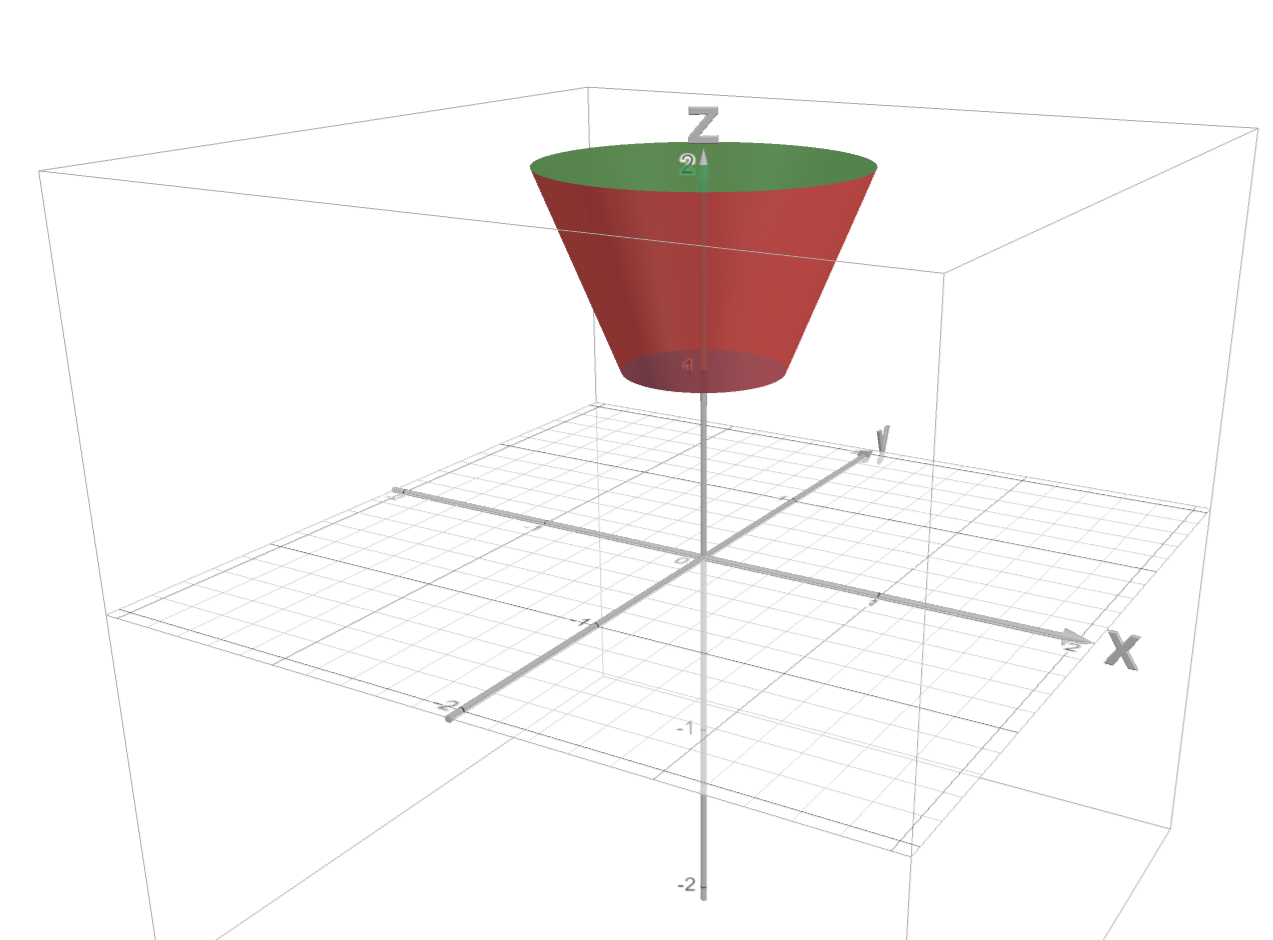
\includegraphics[width=0.5\textwidth]{cone.png}
    \caption{The region $\U$}
    \label{fig:cone}
  \end{figure}
\end{problem}

\newpage

% Vector fields, medium
\begin{problem}
  Let $\BF$ be the vector field $z\bi+x\bj+y\bk$. Let $\br(t)=(x(t),y(t),z(t)),\ a\leq t\leq b$ be any integral curve of $\BF$.
  \begin{enumerate}[(a)]
    \item (5 points) What system of differential equations must $x(t),y(t),z(t)$ satisfy?
    \vfil
    \item (5 points) Show that no matter what integral curve $\br(t)$ is picked for $\BF$, if $\C$ is the directed curve traced out by $\br(t)$ for $a\leq t\leq b$, then we will always have
    \[\int_\C \BF\cdot d\br\geq 0.\]
  \end{enumerate}
\end{problem}

\end{document}
